\documentclass[12pt,halfparskip]{scrreprt} 
\usepackage{ucs}
\usepackage[utf8x]{inputenc} %font
%\usepackage[default,osfigures,scale=1]{opensans} font
\usepackage{DejaVuSansCondensed}
\renewcommand*\familydefault{\sfdefault} %% Only if the base font of the document is to be sans serif
\usepackage[T1]{fontenc}
\usepackage[ngerman]{babel} %german
\usepackage{graphicx} %images
\usepackage[autostyle=true,german=quotes]{csquotes} %quotation
\usepackage{tabularx} %tables

% PAGE MARGINS
\usepackage{geometry}
\geometry{a4paper, top=25mm, left=25mm, right=25mm, bottom=25mm, headsep=10mm, footskip=10mm}

% HEADER AND FOOTER
\usepackage[automark]{scrlayer-scrpage}
\pagestyle{scrheadings}
\clearscrheadfoot
\setfootsepline[\textwidth]{0.5pt}
\ofoot[]{\pagemark}

% DOCUMENT NAMING
\title{Dokumentation Fallbeispiel}
\subtitle{DVD Archiv}
\author{Jasmin Thevathas, Marc Hutzli, Robin Schmid\\JARCHITECTS}
\date{29. Januar in Burgdorf}	

% VARIABLES FOR TITLE PAGE
\makeatletter
\let\title\@title
\let\author\@author
\let\date\@date
\let\subtitle\@subtitle
\makeatother

% THE DOCUMENT
\begin{document}

% TITLEPAGE
\begin{titlepage}
    \begin{center}
        \vspace*{1cm}
        
        \Huge{\textbf{\title}}\\
        \vspace{2cm}
        \LARGE{\subtitle}

        \vspace{1.5cm}
        
        \large{\author}
        
        \vspace{1.5cm}

        \large{\date}
        \vfill
        
        \vspace{0.8cm}
                
    \end{center}
\end{titlepage}

\tableofcontents


\chapter{Einführung}
\label{chap:introduction}
Dieses Dokument dient zum besseren Verständnis unseres Projekts respektive Fallbeispiels im Modul \enquote{Java Soft. Entwicklung mit Open Source 1}. 

%
%\begin{figure}[h]
%	\centering
%	\includegraphics[width=0.75\textwidth]{systemkontext_projekt2}
%	\caption{Vereinfachtes Schema des Systemkontexts}
%\end{figure}
\chapter{Domain Model}
\label{chap:domainmodel}

\begin{figure}[h]
	\centering
	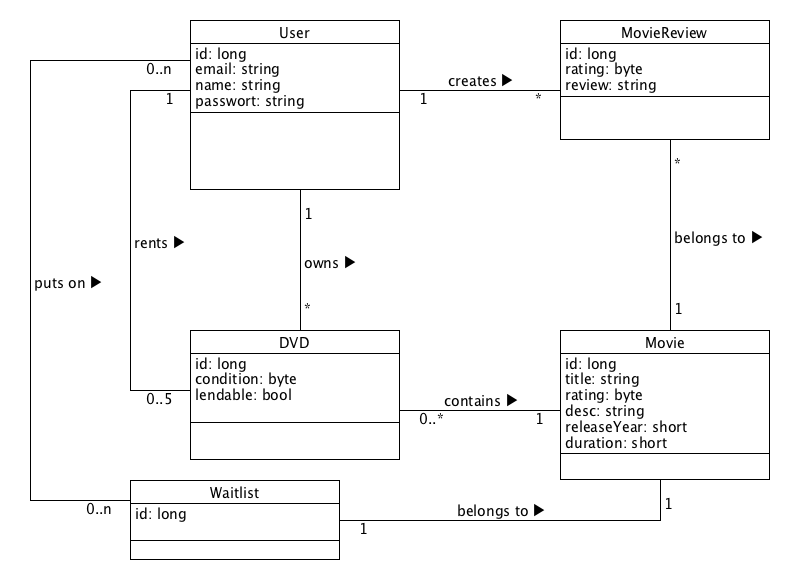
\includegraphics[width=1\textwidth]{img/domain_model.png}
	\caption{Erste Version des Domain Models}
\end{figure}

\section{Übersicht}
In einer ersten Phase wurde 

Die finale Version des Domain Models sehen Sie in Abbildung \ref{fig:domainmodel}.

\section{Entitäten}

\minisec{User}
Beschreibt einen Benutzer des Systems. Er besitzt einen Namen, E-Mail Adresse und ein Passwort. Ausserdem kann er Besitzer (\emph{owns}) von mehreren \textbf{DVD}s sein.

\minisec{DVD}

\minisec{Movie}

\minisec{MovieReview}

\minisec{RentRecord}

\minisec{ReservationRecord}

\begin{figure}[h]
	\centering
	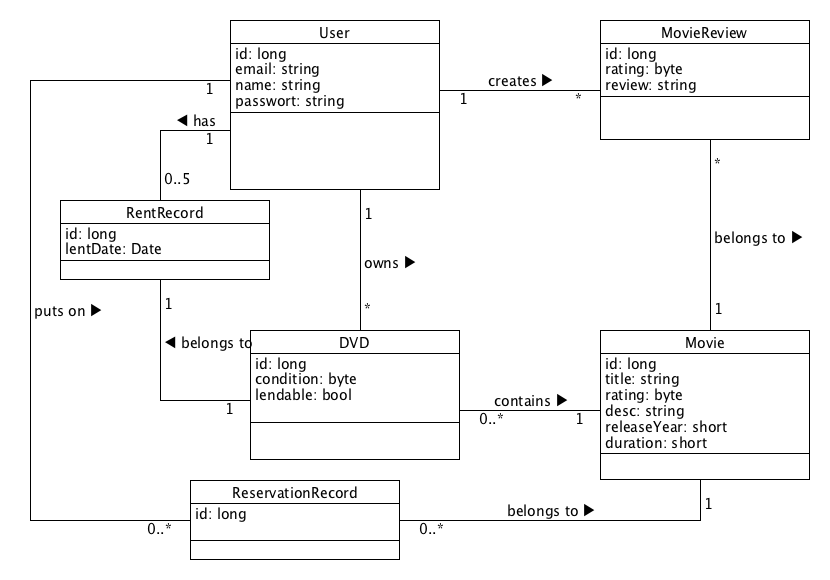
\includegraphics[width=1\textwidth]{img/domain_model2.png}
	\caption{Finale Version des Domain Models}
	\label{fig:domainmodel}
\end{figure}


\chapter{Ziel}
\label{chap:ziel}

\section{Hauptziel}
Das Hauptziel ist, dass nach Beendigung des Projektes ein Machbarkeitsnachweis für ein Game bereitgestellt ist, welches Mehrspielerfähig ist, wobei mobile Devices per Browser als Spielcontroller fungieren.

Weitere Informationen finden Sie im Kapitel \ref{chap:ziel} auf Seite \pageref{chap:ziel}.


\begingroup
\setlength{\tabcolsep}{10pt} % Default value: 6pt
\renewcommand{\arraystretch}{1.5}
\section{Unterziele}
\begin{tabularx}{\textwidth}{ |l|X| }
  \hline
  \textbf{Z 1}	& \textbf{Wirtschaftliche Ziele}	\\	\hline
  Z 1.1	& Der Entwicklungsaufwand für ein umgesetztes System ist bekannt.  	\\	\hline
  Z 1.2	& Die Betriebskosten für ein umgesetztes System ist bekannt.  	\\	\hline
  Z 1.3	& Es liegt eine Beurteilung des Marktpotentials vor.  	\\	\hline
  \hline
  \textbf{Z 2}	& \textbf{Technische Ziele}	\\	\hline
  Z 2.1	& Es ist eine Hardware evaluiert, die für das System hinreichend ist.  	\\	\hline
  Z 2.2	& Es existiert ein Software Prototyp, der die Nutzlast testen lässt.  	\\	\hline
  Z 2.3	& Die Eignung möglicher Frameworks für die Umsetzung wurde geprüft.	\\	\hline
  \hline
  \textbf{Z 3}	& \textbf{Konzeptionelle Ziele}	\\	\hline
  Z 3.1	& Es existieren graphische Entwürfe für den Einsatz des Systems. 	\\	\hline 
  
  \hline
  \textbf{Z 4}	& \textbf{Ziele aus Anforderungsmanagement}	\\	\hline
  Z 4.1	& Der Systemkontext ist abgegrenzt.	\\	\hline
  Z 4.2	& Die Stakeholder sind definiert.	\\	\hline
  Z 4.3	& Die funktionalen Anforderungen an ein System sind ermittelt.	\\	\hline
  Z 4.4	& Die Qualitätsanforderungen an ein derartiges System sind festgelegt.	\\	\hline
  Z 4.5	& Allfällige Randbedingungen sind evaluiert. 	\\	\hline
\end{tabularx}
\endgroup

\chapter{Setup}

\section{git Repository}
Das Repository des Projektes ist zu finden unter:\\

\textbf{https://github.com/tjasmin21/ch.bfh.jarchitects.filmbiblio.boot}
\\

Der aktuelle Entwicklungsbranch ist \emph{jasmin}.

\section{Setup-Anleitung}

\begin{enumerate} 
	\item mkdir dvdarchiv \&\& cd dvdarchiv
	\item git clone \emph{repo-link} .
	\item git checkout jasmin
	\item mvn install
	\item Projekt in IDE öffnen und runnen
	\item localhost:8080 im Browser öffnen
	\item Bier öffnen!
\end{enumerate}

\end{document}